% Options for packages loaded elsewhere
\PassOptionsToPackage{unicode}{hyperref}
\PassOptionsToPackage{hyphens}{url}
%
\documentclass[
  12pt,
]{article}
\usepackage{lmodern}
\usepackage{amsmath}
\usepackage{ifxetex,ifluatex}
\ifnum 0\ifxetex 1\fi\ifluatex 1\fi=0 % if pdftex
  \usepackage[T1]{fontenc}
  \usepackage[utf8]{inputenc}
  \usepackage{textcomp} % provide euro and other symbols
  \usepackage{amssymb}
\else % if luatex or xetex
  \usepackage{unicode-math}
  \defaultfontfeatures{Scale=MatchLowercase}
  \defaultfontfeatures[\rmfamily]{Ligatures=TeX,Scale=1}
  \setmainfont[]{Times New Roman}
\fi
% Use upquote if available, for straight quotes in verbatim environments
\IfFileExists{upquote.sty}{\usepackage{upquote}}{}
\IfFileExists{microtype.sty}{% use microtype if available
  \usepackage[]{microtype}
  \UseMicrotypeSet[protrusion]{basicmath} % disable protrusion for tt fonts
}{}
\makeatletter
\@ifundefined{KOMAClassName}{% if non-KOMA class
  \IfFileExists{parskip.sty}{%
    \usepackage{parskip}
  }{% else
    \setlength{\parindent}{0pt}
    \setlength{\parskip}{6pt plus 2pt minus 1pt}}
}{% if KOMA class
  \KOMAoptions{parskip=half}}
\makeatother
\usepackage{xcolor}
\IfFileExists{xurl.sty}{\usepackage{xurl}}{} % add URL line breaks if available
\IfFileExists{bookmark.sty}{\usepackage{bookmark}}{\usepackage{hyperref}}
\hypersetup{
  pdftitle={Insert title of project here},
  pdfauthor={Name},
  hidelinks,
  pdfcreator={LaTeX via pandoc}}
\urlstyle{same} % disable monospaced font for URLs
\usepackage[margin=2.54cm]{geometry}
\usepackage{graphicx}
\makeatletter
\def\maxwidth{\ifdim\Gin@nat@width>\linewidth\linewidth\else\Gin@nat@width\fi}
\def\maxheight{\ifdim\Gin@nat@height>\textheight\textheight\else\Gin@nat@height\fi}
\makeatother
% Scale images if necessary, so that they will not overflow the page
% margins by default, and it is still possible to overwrite the defaults
% using explicit options in \includegraphics[width, height, ...]{}
\setkeys{Gin}{width=\maxwidth,height=\maxheight,keepaspectratio}
% Set default figure placement to htbp
\makeatletter
\def\fps@figure{htbp}
\makeatother
\setlength{\emergencystretch}{3em} % prevent overfull lines
\providecommand{\tightlist}{%
  \setlength{\itemsep}{0pt}\setlength{\parskip}{0pt}}
\setcounter{secnumdepth}{5}
\ifluatex
  \usepackage{selnolig}  % disable illegal ligatures
\fi
\newlength{\cslhangindent}
\setlength{\cslhangindent}{1.5em}
\newlength{\csllabelwidth}
\setlength{\csllabelwidth}{3em}
\newenvironment{CSLReferences}[2] % #1 hanging-ident, #2 entry spacing
 {% don't indent paragraphs
  \setlength{\parindent}{0pt}
  % turn on hanging indent if param 1 is 1
  \ifodd #1 \everypar{\setlength{\hangindent}{\cslhangindent}}\ignorespaces\fi
  % set entry spacing
  \ifnum #2 > 0
  \setlength{\parskip}{#2\baselineskip}
  \fi
 }%
 {}
\usepackage{calc}
\newcommand{\CSLBlock}[1]{#1\hfill\break}
\newcommand{\CSLLeftMargin}[1]{\parbox[t]{\csllabelwidth}{#1}}
\newcommand{\CSLRightInline}[1]{\parbox[t]{\linewidth - \csllabelwidth}{#1}\break}
\newcommand{\CSLIndent}[1]{\hspace{\cslhangindent}#1}

\title{Insert title of project here}
\usepackage{etoolbox}
\makeatletter
\providecommand{\subtitle}[1]{% add subtitle to \maketitle
  \apptocmd{\@title}{\par {\large #1 \par}}{}{}
}
\makeatother
\subtitle{Web address for GitHub repository}
\author{Name}
\date{}

\begin{document}
\maketitle

\newpage

\hypertarget{rationale-and-research-questions}{%
\section{Rationale and Research
Questions}\label{rationale-and-research-questions}}

While many of the rivers we've examined over the course of the semester
are in North Carolina and have discharge levels driven primarily by
precipitation, many rivers in the western U.S. are heavily influenced by
runoff from snowpack and their discharges are more seasonal. The
relationship between snowpack, measured as snow-water equivalent (SWE),
and discharge is less direct than precipitation and discharge, and often
influenced by a number of other factors. My project explores two
questions:

\begin{itemize}
\tightlist
\item
  What is the relationship between peak SWE and peak discharge in terms
  of magnitude and timing?
\item
  How has the lag time between peak snowpack and peak runoff change over
  time?
\end{itemize}

\newpage

\hypertarget{dataset-information}{%
\section{Dataset Information}\label{dataset-information}}

\newpage

\hypertarget{methodology}{%
\section{Methodology}\label{methodology}}

Look at cal year bc max SWE occurs in April and max discharge occurs in
summer.

\newpage

\hypertarget{exploratory-analysis}{%
\section{Exploratory Analysis}\label{exploratory-analysis}}

Discharge on the Animas River is very seasonal, typically characterized
by peaks in the months of May and June due to runoff from snowmelt
(Figure 1). A Mann-Kendall test shows that discharge on the Animas has
been decreasing significantly since 1987 (p \textless{} 0.05).

\begin{figure}
\centering
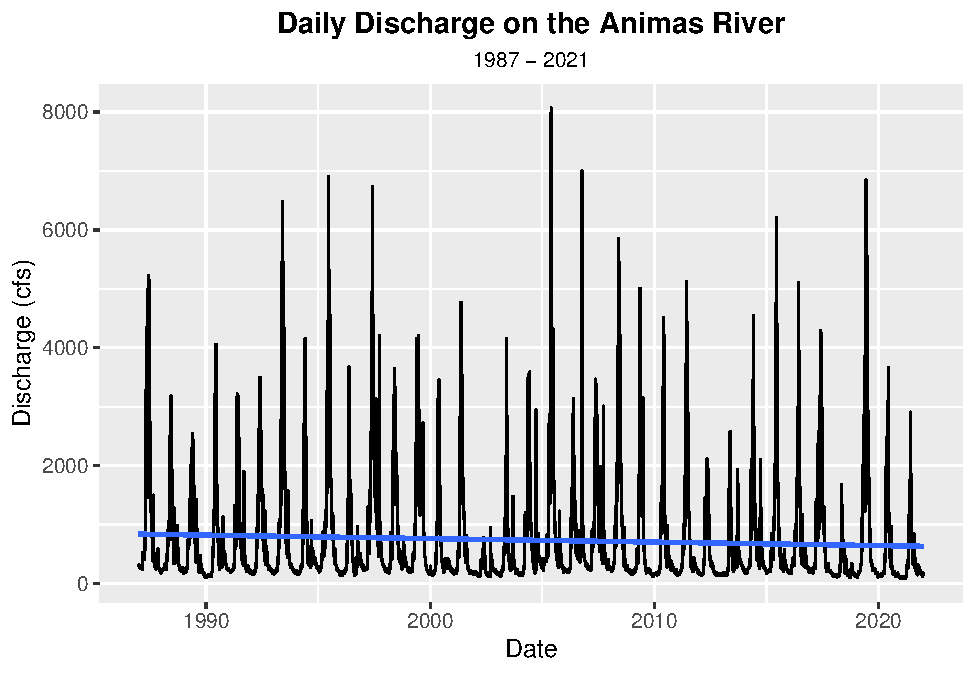
\includegraphics{Final_Report_files/figure-latex/unnamed-chunk-1-1.pdf}
\caption{Daily discharge measured in cubic feet per second on the Animas
River at Durango, Colorado}
\end{figure}

The seasonality of SWE in the mountains above Durango generally mirrors
that of discharge in the Animas River (Figure 2), although peak SWE
occurs 54 days prior to peak discharge on average. a Mann-Kendall test
reveals that SWE has also been decreasing during the same period. It is
unsurprising that both levels of discharge and SWE have decreased from
1987-2021: a new study reveals that ``2000-2021 was the driest 22-yr
period since at least 800'' {[}WILLIAMS2022232{]}.

\begin{figure}
\centering
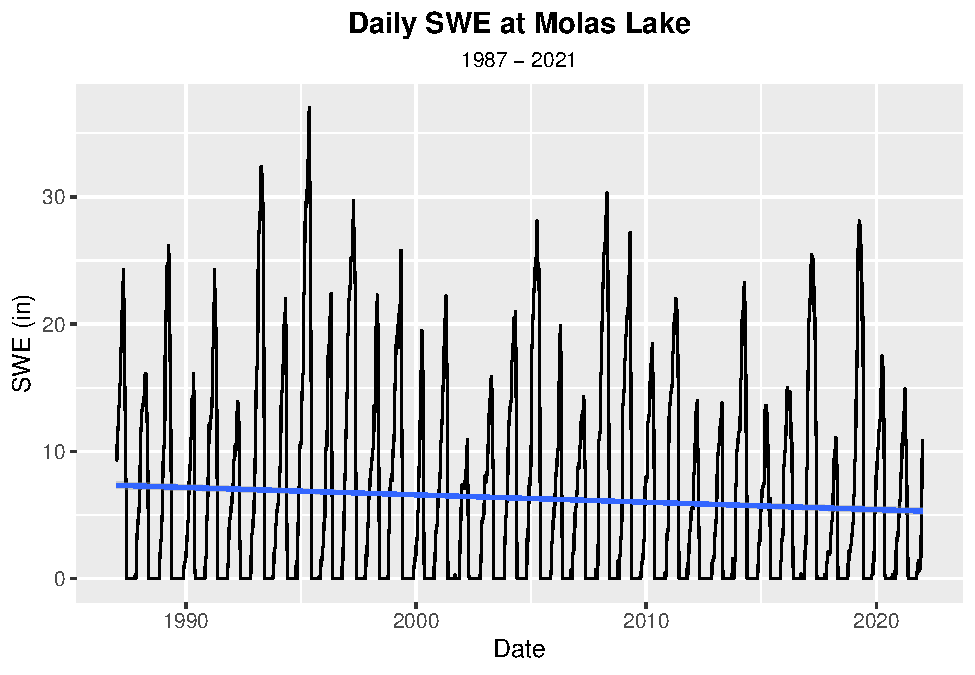
\includegraphics{Final_Report_files/figure-latex/unnamed-chunk-2-1.pdf}
\caption{Snow water equivalent at Molas Lake, upstream of the Animas
River USGS gage in Durango}
\end{figure}

\newpage

\hypertarget{analysis}{%
\section{Analysis}\label{analysis}}

\hypertarget{question-1-what-is-the-relationship-between-peak-swe-and-peak-discharge-in-terms-of-magnitude-and-timing}{%
\subsection{Question 1: What is the relationship between peak SWE and
peak discharge in terms of magnitude and
timing?}\label{question-1-what-is-the-relationship-between-peak-swe-and-peak-discharge-in-terms-of-magnitude-and-timing}}

\hypertarget{question-2-how-has-the-lag-time-between-peak-snowpack-and-peak-runoff-change-over-time}{%
\subsection{Question 2: How has the lag time between peak snowpack and
peak runoff change over
time?}\label{question-2-how-has-the-lag-time-between-peak-snowpack-and-peak-runoff-change-over-time}}

\newpage

\hypertarget{summary-and-conclusions}{%
\section{Summary and Conclusions}\label{summary-and-conclusions}}

\newpage

\hypertarget{references}{%
\section{References}\label{references}}

\textless add references here if relevant, otherwise delete this
section\textgreater{}

\hypertarget{refs}{}
\begin{CSLReferences}{1}{0}
\leavevmode\hypertarget{ref-WILLIAMS2022232}{}%
A. Park Williams, J. E. S., Benjamin I. Cook. (2022). Rapid
intensification of the emerging southwestern north american megadrought
in 2020--2021. \emph{Nature Climate Change}, \emph{12}, 232--234.
https://doi.org/\url{https://doi.org/10.1016/j.landurbplan.2013.12.008}

\end{CSLReferences}

\end{document}
